\chapter{Experimental evaluation}
\label{chap:evaluation}

We compare the benchmarking methods on multiple experiments in multiple environments.
All experiments were run on super-harness described in~\cref{chap:impl}.
This super harness executes A/A benchmarks from multiple benchmark suites using sequential, synchronous and asynchronous duet benchmarking methods.

\section{Experiment setup}
\label{sec:experiment_setup}

Benchmark suites used in the experiments are Renaissance, ScalaBench, DaCapo, and SPEC CPU 2017.
Latter three are also part of~\citet{bulej2020duet} and two of those --- ScalaBench and DaCapo are representatives of synchronous duet method as their harnesses were adapted to work with \lstinline{duetbench}.

Renaissance benchmark suite was selected as a modern JVM suite with a focus on parallel workloads among others\cite{prokopec2019renaissance}.
We used version $0.13$ and had to exclude \lstinline{neo4j-analytics} benchmark as it failed to execute on our configuration.

ScalaBench~($v.9.12$) and DaCapo~($v.9.12$) are both JVM benchmarks that have significant overlap in benchmarks but are the only ones that have their runtime altered to run synchronous duet.
For DaCapo and ScalaBench we excluded \lstinline{batik}, \lstinline{eclipse}, \lstinline{tomcat}, \lstinline{actors}, and \lstinline{jython} (the last two are only in ScalaBench).
Both suites were run with \lstinline{--novalidation} parameter to tighten the workload loop.

All Java benchmarks were run in OpenJDK 11.0.11 JVM with fixed heap size and disabled garbage collection ergonomics, other virtual machine settings were left at their defaults.

SPEC CPU 2017 is the sole non-Java benchmark --- representative of natively compiled C, C++, and Fortran benchmarks.
We run its rate workloads in peak tuning using the \lstinline{onlyrun} action\footnote{Disclaimer: SPEC CPU prohibits publications of results without verification, but for our use-case verification could affect our results negatively, and we don't report SpecCPU score just use the iteration durations.} that skips additional non-workload steps.
SPEC CPU was not intended to run in a container and hence we faced multiple issues setting it up.
From build and training errors in installation step (\lstinline{503.bwaves_r}, \lstinline{510.parest_r}, \lstinline{521.wrf_r}, \lstinline{527.cam4_r}) to runtime memory requirements (\lstinline{502.gcc_r}, \lstinline{523.xalancbmk_r}, \lstinline{526.blender_r}).
Overall we run 14 benchmarks from SPEC CPU 2017.

\subsection{Docker setup}
Docker image for Renaissance suite is based on \lstinline{renaissancebench/buildenv:openj9-openjdk11}~\footnote{\url{https://hub.docker.com/r/Renaissancebench/buildenv}}, ScalaBench and DaCapo images are based on \lstinline{openjdk:11.0.8-jdk}~\footnote{\url{https://hub.docker.com/_/openjdk}} image, but it is adjusted to run synchronization agent described in~\cref{sec:sync_duet_impl}.
The Docker image for SpecCPU is based on \lstinline{ubuntu} image and the whole suite installation is done in the container build step using a configuration with \lstinline{gcc}, the full configuration is available in the attached source code.

Docker containers run with no additional options than mentioned in~\cref{chap:impl}.
In particular, there are no reservations on CPU or memory.
There are multiple reasons for this (1) benchmarks themselves check the number of available CPUs and set their parallelism accordingly, but that information is returned by the OS and thus would same for both duet pairs regardless of docker allocations, (2) the CPU reservations would rule out use of smaller cloud instances, (3) impact symmetry with completely fair scheduler should allocate equal resources to both benchmarks, hence simplifying setup.

\subsection{Run summary}

One of the goals of the duet methods is to enable benchmarking in varying environments:
\begin{description}
	\item[cloud] environments is represented by AWS EC2 \lstinline{t3.medium} instances,
	\item[bare-metal] environment consist of dedicated \mbox{bare-metal} servers,
	\item[shared-VM] environment is \mbox{self-hosted} virtualized environment with no special performance measurement treatment that is actively used by other students.
\end{description}
AWS \lstinline{t3.medium} instance was chosen because the \lstinline{t2} instances were not powerful enough to run two SPEC CPU benchmarks in docker side by side and \lstinline{t3.medium} turned out to be the cheapest alternative able to do so.
The measurements were parallelized across multiple instances in each environment except for the school \mbox{shared-VM} environment as there is only one instance.
\Cref{table:envs} summarizes the configuration of selected platforms and the timeframe of the measurements.

\begin{table}[ht]
  \centering
  \resizebox{\textwidth}{!}{\begin{tabular}{llllll}
  Environment   & Instances & CPU                                                                     & vCPUs & Memory  & Measurements \\
  \hline
  AWS t3.medium & 10        & \begin{tabular}[c]{@{}l@{}}Intel(R) Xeon(R) Platinum 8259CL\\
		                                                 Intel(R) Xeon(R) Platinum 8175M\end{tabular} & 2     & 4.0 GiB & Jul 12 -- Jul 19 2022\\
  \\
  Bare metal    & 8         & Intel(R) Xeon(R) CPU E3-1230 v6                                         & 4     & 32 GiB  & \begin{tabular}[c]{@{}l@{}}Jun 17 -- Jun 22 2022\\
                                                                                                                                                     Dec 8 -- Dec 10 2022\end{tabular}\\
  \\
  Teaching      & 1         & Intel(R) Xeon(R) CPU E5-2620 v4                                         & 4     & 16 GiB  & Dec 3 -- Dec 20 2022
  \end{tabular}}
  \caption{Summary of selected platforms.}
  \label{table:envs}
\end{table}

We ran 20 runs of each benchmark in each environment with every available measurement type.
The only exception is the \mbox{shared-VM} environment where we decided not to run SPEC CPU due to disk and runtime requirements.
That sums up to more than 100 days of machine time executing 61 unique benchmarks.

Each benchmark run has been executed for a given amount of iterations or until it reached a timeout.
Timeout for \mbox{Java-based} benchmarks was 5 minutes and for SPEC CPU it was 30 minutes.
The iteration limit for Renaissance was set to default which is supposed to be reasonable for that type of benchmark.
ScalaBench and DaCapo had hard a limit of 50 iterations while SPEC CPU only 10.
Deep dive into runtime is in the next section.

\section{Measurements}
\label{sec:measurements}

The following sections provide answers to research questions proposed in~\cref{chap:duet}.
Often, due to a big number of benchmarks, we aggregate the results by suites or measurement methods.
For detailed --- per benchmark results look into the attached python notebooks described in~\cref{sec:automation}.
All data in the following figures are subject to data preprocessing described in~\cref{sec:data_filtering} unless stated otherwise.

\subsection{RQ1: Runtime savings}
\label{sec:rq1}

The first research question is meant to answer whether the duet methods have overall runtime savings compared to the sequential method.
The presumption is that since duets run concurrently they can be twice as fast as the sequential method which runs one by one.

Runtime is computed on raw measurements, from the start of the particular run to its end. For the sequential method since pairs don't run in parallel add the duration of pairs A and B.
For duet, methods take a sooner start and a later end of a run to compute the duration.
\begin{align*}
runtime^{e, b}_{seqn}  =&~\{end(R^A) - start(R^A) + end(R^B) - start(R^B)~|\\
                        &~~(R^A, R^B) \in M^{e, b}_{seqn}\} \\
runtime^{e, b}_{aduet} =&~\{min(start(R^A), start(R^B)) - max(end(R^A), end(R^B))~|\\
                        &~~(R^A, R^B) \in M^{e, b}_{aduet}\}
\end{align*}

Then runtime speedup for particular benchmark $b \in B$ in an environment $e \in E$:
\begin{equation}\label{eq:runtimespeedup}
runtime\_speedup^{e, b} = \frac{mean(runtime^{e, b}_{seqn})}{mean(runtime^{e, b}_{aduet})}.
\end{equation}

\Cref{fig:runtime_speedup} shows what was the runtime speedup of asynchronous duet run.
As it turns out this is heavily dependent on the environment and on the type of benchmark.
Some benchmarks are indeed almost twice as fast, especially from the SPEC CPU suite in stable environments.
However, there is significant variability and even in the \mbox{bare-metal} environment some benchmarks show no speedup at all, in cloud duet is even slower for some benchmarks.
This is likely the cause of vCPU discrepancy as \lstinline{t3.medium} has only $2$ vCPUs while other environments have $4$.

Overall, the median speedup is $5\%$, $73\%$, and $53\%$ for cloud, bare-metal, and shared-VM environments respectively.
These results show that using duet methods can significantly reduce the machine time required to run benchmarks.

\begin{figure}
	\centering
	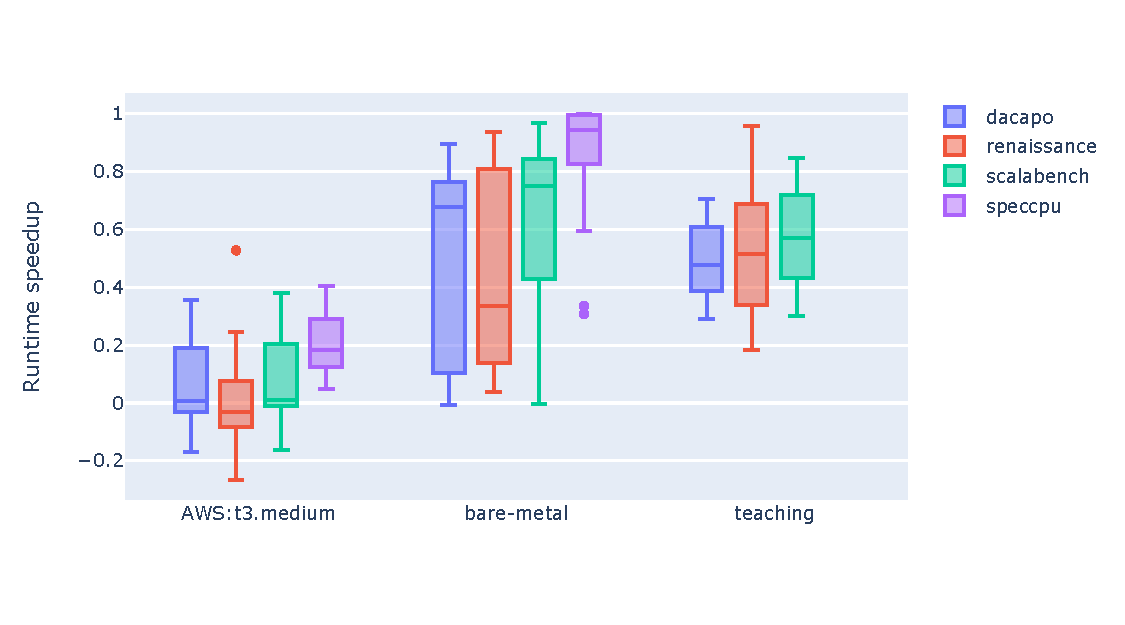
\includegraphics[width=.9\linewidth]{./figures/runtime_speedup.pdf}
	\caption{
		Runtime speedup of asynchronous duet method across different environments and suites.
		This is not subject to data preprocessing from~\cref{sec:data_filtering} as it captures raw measurements time.
	}
	\label{fig:runtime_speedup}
\end{figure}

\subsection{RQ2: Pair overlaps}
\label{sec:rq2}

The second research question aims to understand the nature of asynchronous duet iteration overlaps.
However, as stated in~\cref{sec:overlaps}, not all overlaps are the same.
It is especially important for the CI computation from~\ref{sec:ci_test} where the minimum overlap rate is used for pairing asynchronous duet iterations.
Formally, for benchmark $b \in B$ in environment $e \in E$ and minimum overlap ratio $m$
$$
relative\_overlap\_time^{e, b}_m = \frac{\sum\limits_{(i^A, i^B) \in O^{e,b}_m} 2 * overlap\_time(i^A, i^B)}{\sum\limits_{(R^A, R^B) \in M^{e, b}_{aduet}}(\sum\limits_{i \in R^A} i + \sum\limits_{i \in R^B} i)}.
$$
The overlap time in the nominator is doubled because the overlap is symmetric relation and the denominator accounts for the runtime of both pairs, this way the $relative\_overlap\_time^{e, b}_m \in [0, 1]$ and represents a percentage of overlapping workload runtime, not just a harness.

\Cref{fig:relative_overlap_time} shows how much does minimum overlap rate affect the relative overlap time.
SPEC CPU has very good overlap coverage which suggests a low variance of iteration durations.
Other suites show a steady decline as the minimum overlap ratio reaches $90\%$ overlap time is less than $20\%$ of total iteration time hindering the runtime improvements from~\cref{sec:rq1}.
However, the minimum overlap ratio of $30\%$ or $50\%$ retains above $80\%$ or $60\%$ of iteration runtime respectively, which seems like a good fit for the minimum overlap ratio parameter.

\begin{figure}
	\centering
	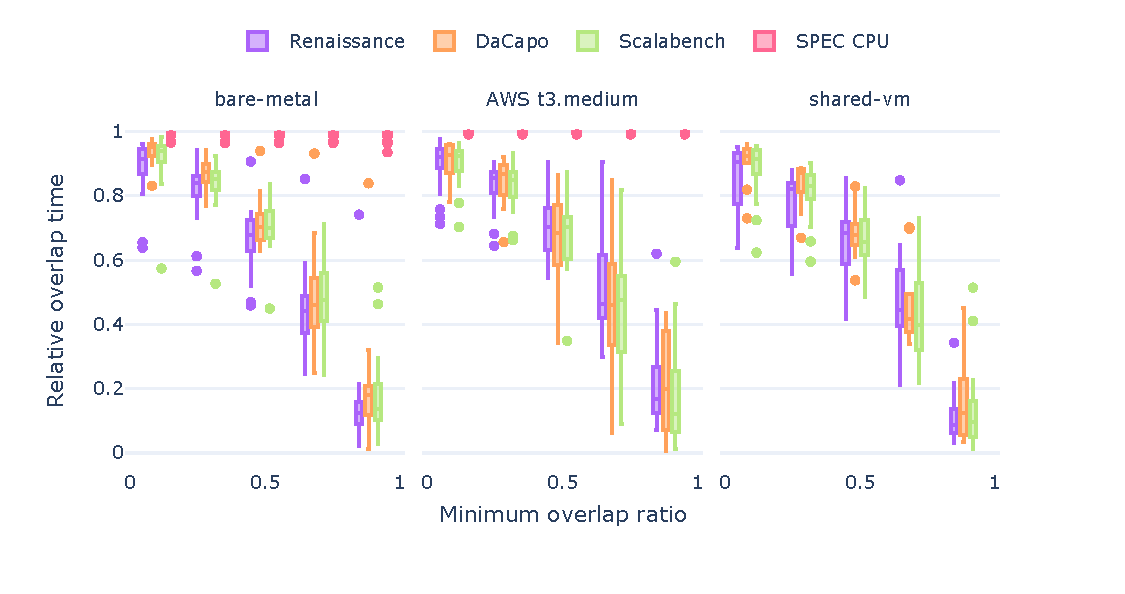
\includegraphics[width=1\linewidth]{./figures/relative_overlap_time.pdf}
	\caption{
		Box plot of benchmarks in respective suites that describes how big is the relative overlap time of these benchmarks compared to overall iteration time with different minimum overlap rates.
	}
	\label{fig:relative_overlap_time}
\end{figure}

\xxx{TODO: Include examples of some overlap length distributions. Consider including lag some lag plots that would show synchronized nature of overlaps.}

\subsection{RQ3: Accuracy improvements}
\label{sec:rq3}

The third research question concerns the accuracy of regression detection using different benchmarking methods across different environments.
The accuracy is inherently dependent on the variance of measurements.
Therefore, the first method of comparison uses relative standard deviation $CV$ as described in~\cref{sec:cv}.

\Cref{fig:cv} shows $CV$ of different benchmarking methods across different environments for all benchmarks.
It shows that duet methods have comparable variance and even though the sequential method has usually smaller $CV$ in all environments there is no significant difference between methods nor environments.
SPEC CPU has the smallest $CV$ which is expected since it is the only natively compiled suite with longer runtime.
A closer look shows common benchmark outliers, namely \lstinline{luindex} in the \mbox{shared-VM} environment in both ScalaBench and DaCapo suites, \lstinline{fop} from DaCapo in \mbox{shared-VM} and cloud environments, and the \lstinline{dotty} from Renaissance suite in the cloud environment which has maximum $CV$ of $0.8$.

\begin{figure}
	\centering
	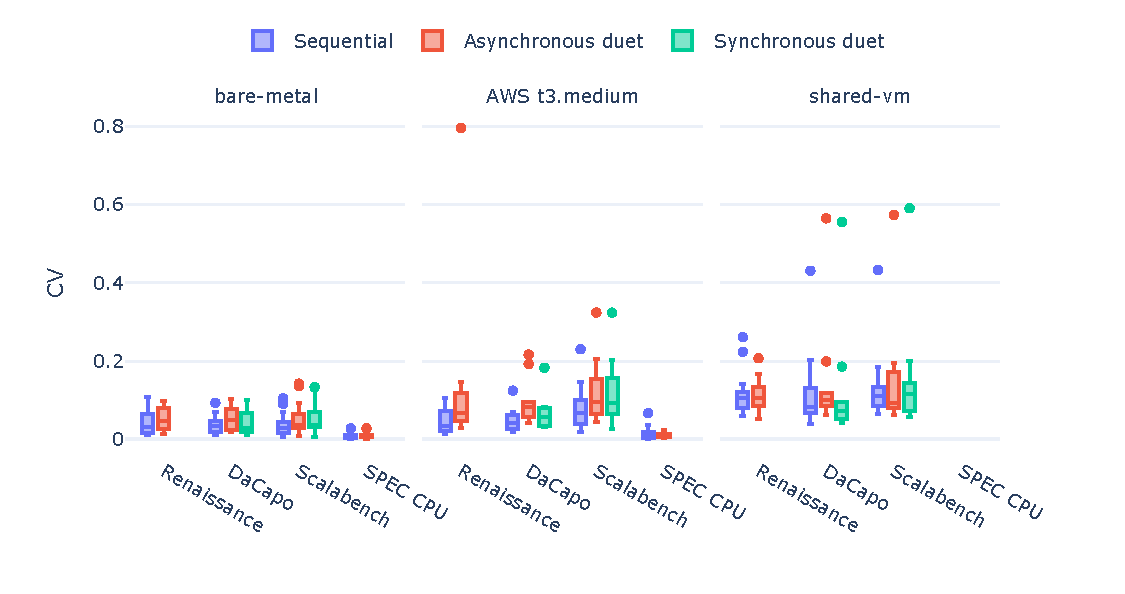
\includegraphics[width=1\linewidth]{./figures/cv.pdf}
	\caption{
		Box plot of benchmarks from respective suites and their $CV$ for different benchmarking methods and environments.
	}
	\label{fig:cv}
\end{figure}

Next, we can determine the accuracy of each method using A/A detection correctness of CI test from~\cref{sec:ci_test}.
As shown in~\cref{sec:rq2} the value of the minimum overlap ratio can significantly influence overall overlap time.
\Cref{fig:citest_overlap_aa} shows success of CI test in determining A/A run based on minimum overlap ratio.
The first important takeaway is that the CI test has reasonably good A/A detection capabilities across all environments.
However, steep rises or declines imply that multiple benchmarks in the given suite were on the edge of CI straddling $0$ which is expected as higher values of minimum overlap ratio decrease the overlap runtime significantly~\ref{fig:relative_overlap_time}.

ScalaBench in the \mbox{shared-VM} environment comes the off worst with only $70\%$ A/A detection rate closely followed by SPEC CPU with only $81\%$.
The low correctness of the CI test for the SPEC CPU suite is likely a result of its low variance and small relative CI width as shown in~\cref{fig:ci_width}.
Based on these findings we set the minimum overlap ratio to $40\%$ in the following CI computations.

\begin{figure}
	\centering
	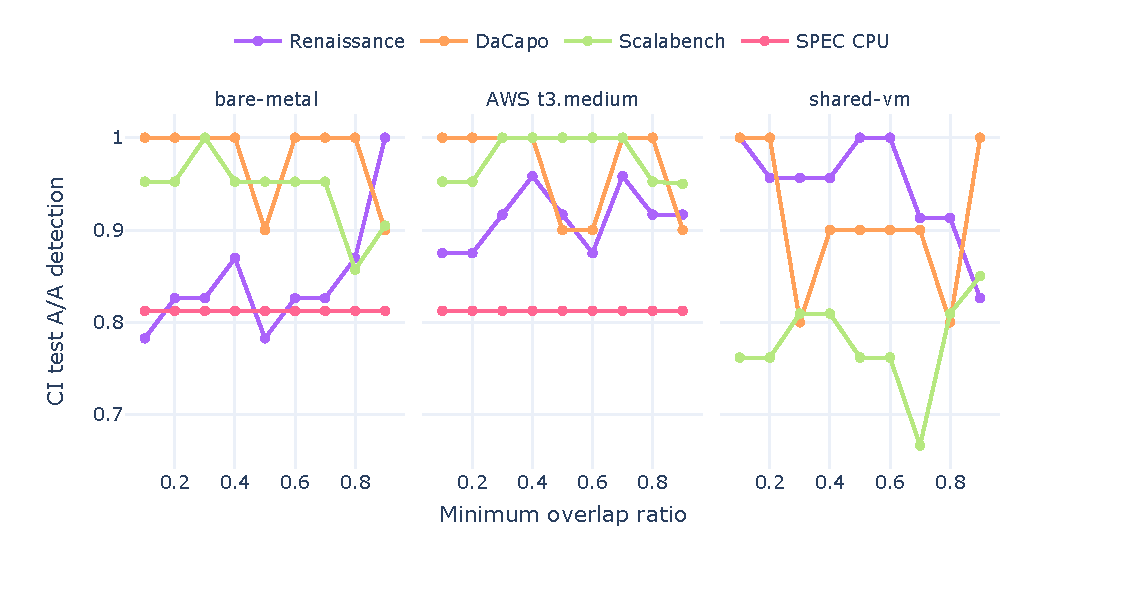
\includegraphics[width=1\linewidth]{./figures/citest_aa_match_by_overlap.pdf}
	\caption{
		The effect of asynchronous duet overlap ratio on correct A/A run detection using the CI test.
		Note that each suite has a different amount of benchmarks.
	}
	\label{fig:citest_overlap_aa}
\end{figure}

\Cref{fig:ci_width} shows relative CI width~\ref{sec:ci_width}.
The width of CI compares iteration variance across environments and the variance of CI computation in particular.
It differentiates the \mbox{shared-VM} environment despite the fact that all environments had low $CV$~\ref{fig:cv}.
Surprisingly, the CI width for the cloud environment looks very similar to bare metal measurements.

\begin{figure}
	\centering
	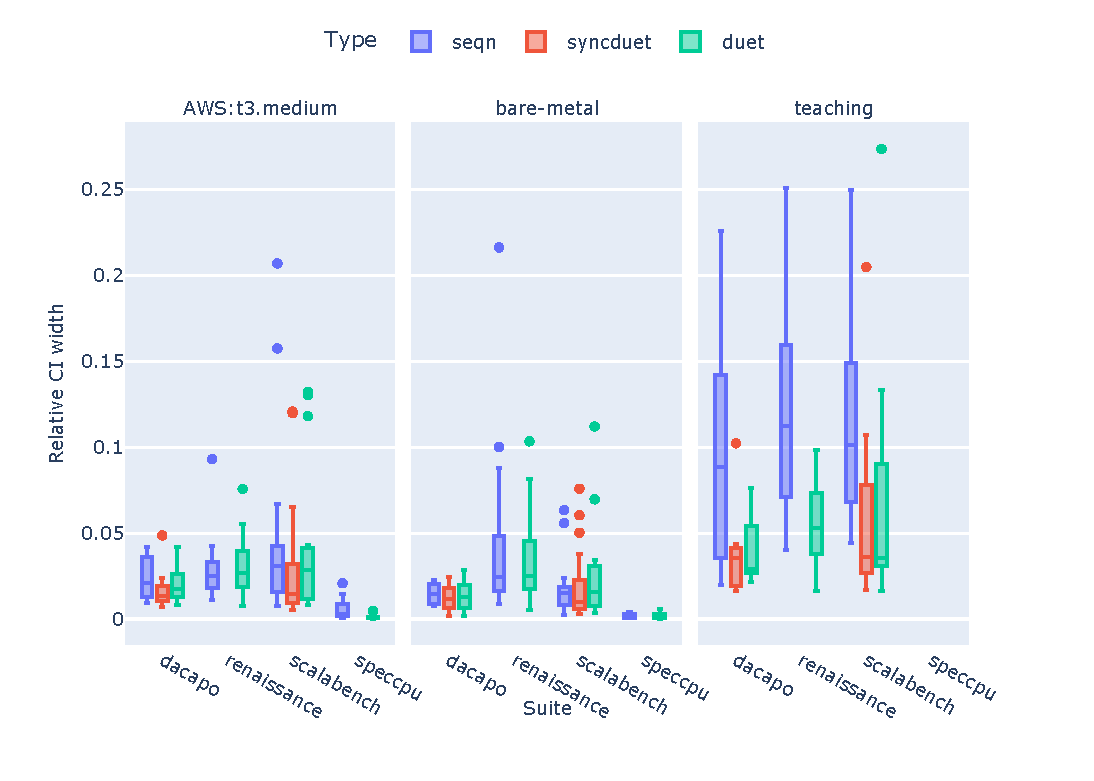
\includegraphics[width=1\linewidth]{./figures/ci_width.pdf}
	\caption{
		Box plot of benchmarks from respective suites and their relative CI width. 
		CI for asynchronous duet uses the minimum overlap ratio of $40\%$.
	}
	\label{fig:ci_width}
\end{figure}

The overall results of the CI test are in \Cref{fig:citest_aa}.
CI test achieves the best results in the cloud environment but the overall correctness of A/A detection straddles $80\%$.
One particular thing to point out is that the sequential method is not worse than duet methods and sometimes even outperforms duet methods.

\begin{figure}
	\centering
	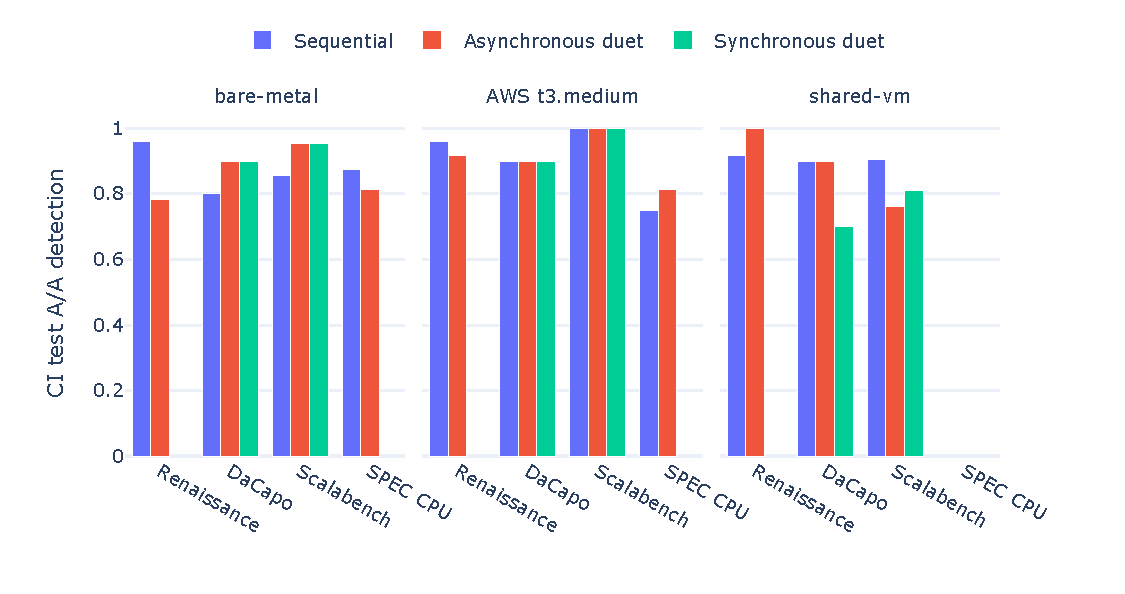
\includegraphics[width=1\linewidth]{./figures/citest_aa_match.pdf}
	\caption{
		The success of the CI test in determining A/A run.
	}
	\label{fig:citest_aa}
\end{figure}

\Cref{fig:utest_aa} shows success of \mbox{u-test} described in~\cref{sec:utest} in determining A/A run.
The \mbox{u-test} seems to be doing much worse compared to the CI test in the \mbox{bare-metal} environment in particular.
However, it has a $100\%$ success rate on the SPEC CPU suite in the cloud environment for both sequential and asynchronous duet methods.

\begin{figure}
	\centering
	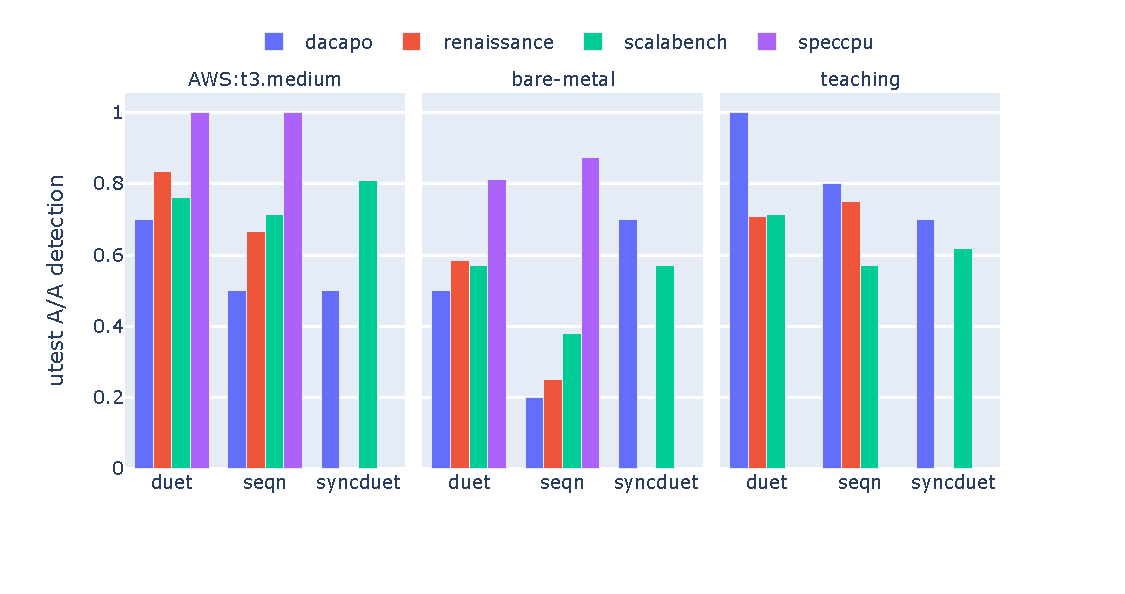
\includegraphics[width=1\linewidth]{./figures/utest_aa_match.pdf}
	\caption{
		The success of \mbox{u-test} in determining A/A run.
	}
	\label{fig:utest_aa}
\end{figure}

\subsection{RQ4: Minimal detectable slowdowns}
\label{sec:rq4}

The last research question regards minimal detectable slowdowns (MDS).
First, the results have to be adjusted as described in~\cref{sec:mds}.
Then evaluate regression detection capabilities using CI test and \mbox{u-test}, with no slowdown the values are the same as in~\cref{fig:citest_aa} and~\cref{fig:utest_aa} for CI test and \mbox{u-test} respectively.
The bigger the slowdown the sooner the A/A match should drop to $0\%$ --- no benchmarks were considered equal in performance.

\Cref{fig:mds_citest} shows MDS using the CI-test.
The SPEC CPU has MDS of $1\%$ slowdown for both benchmarking methods and in both environments but its initial A/A detection is only at approximately $80\%$.
The rest of the benchmarks have fairly similar trends of MDS with the sequential method sometimes lacking slightly behind duet methods.
Overall almost all benchmarks have MDS of $5\%$.

\begin{figure}
	\centering
	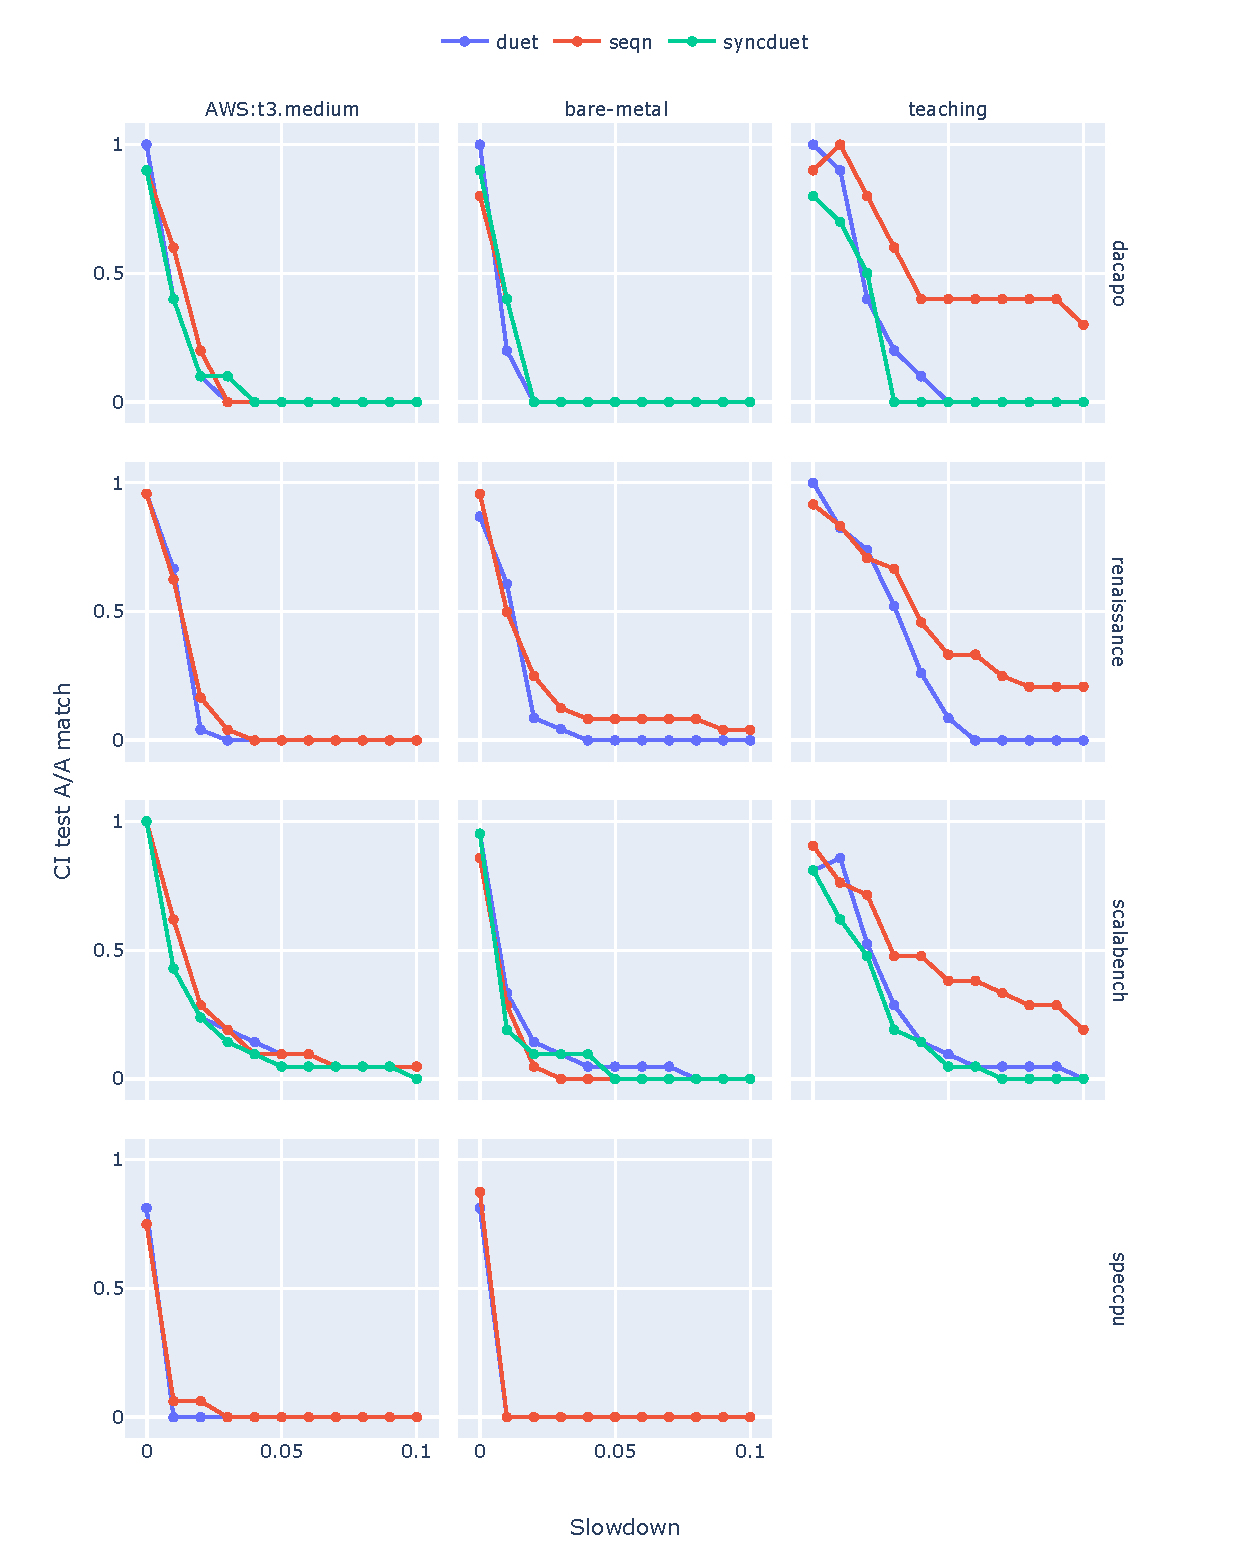
\includegraphics[width=1\linewidth]{./figures/mds_citest.pdf}
	\caption{
    MDS using CI-test.
	}
	\label{fig:mds_citest}
\end{figure}

Since \mbox{u-test} showed a reasonable A/A detection rate only for the SPEC CPU benchmark we showcase MDS for this suite only in~\cref{fig:mds_utest}.
Similar to the CI test, \mbox{u-test} can detect $1\%$ slowdown for the whole SPEC CPU suite.

\begin{figure}
	\centering
	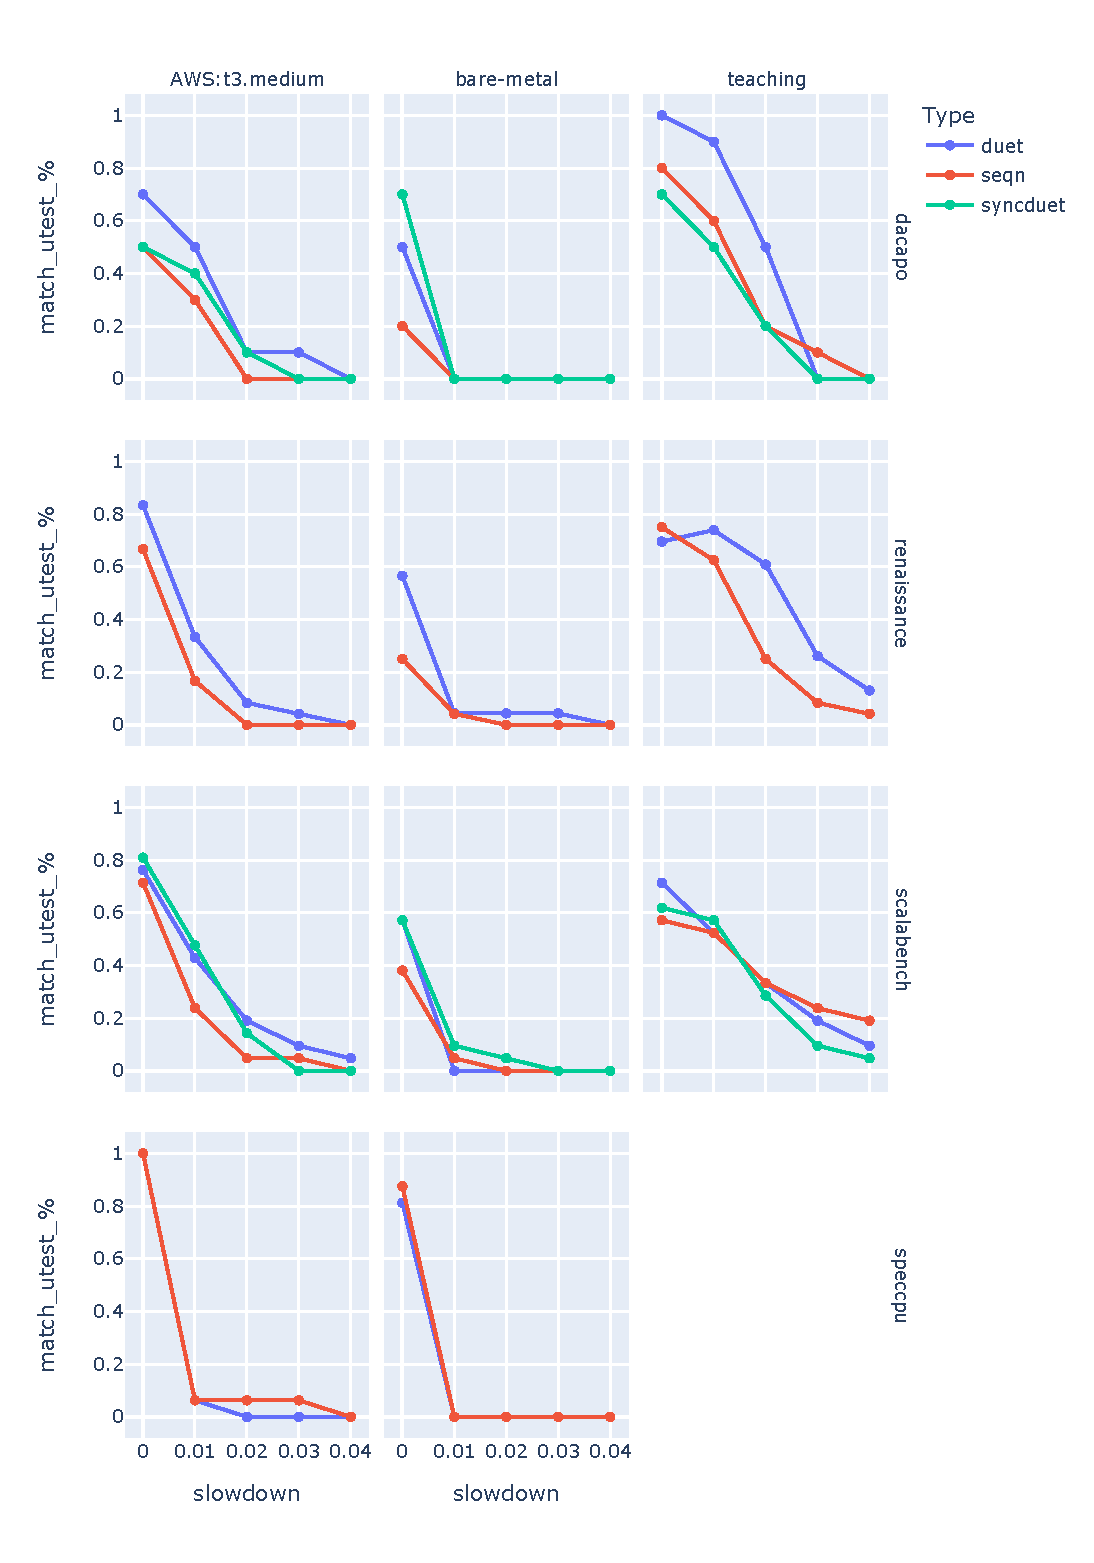
\includegraphics[width=1\linewidth]{./figures/mds_utest.pdf}
	\caption{
    MDS using \mbox{u-test}.
	}
	\label{fig:mds_utest}
\end{figure}

\section{Evaluation automation}
\label{sec:automation}

\xxx{Add a section about how the \lstinline{duetprocess} tool automizes above described evaluation.}
